\documentclass[11pt]{article}
\usepackage[margin=1in]{geometry}
\usepackage[T1]{fontenc}
\usepackage{lmodern}
\usepackage{microtype}
\usepackage{amsmath,amssymb}
\usepackage{booktabs}
\usepackage{graphicx}
\usepackage{xcolor}
\usepackage[numbers,sort&compress]{natbib}
\usepackage[colorlinks=true,linkcolor=black,citecolor={blue!50!black},urlcolor={blue!50!black}]{hyperref}
\usepackage{enumitem}
\setlist{nosep,leftmargin=*}
% generated by paper/make_figures.py; do not edit
\makeatletter
\@namedef{v@base-bpb-quick}{1.748}
\@namedef{v@base-first-hop1}{52.0\%}
\@namedef{v@base-first-min}{15}
\@namedef{v@base-hop0}{38.0\%}
\@namedef{v@base-hop1}{44.0\%}
\@namedef{v@base-hop2}{40.0\%}
\@namedef{v@base-hop4}{38.0\%}
\@namedef{v@base-hop6}{35.0\%}
\@namedef{v@base-hop8}{21.0\%}
\@namedef{v@base-hours}{1.3}
\@namedef{v@base-steps}{3,269}
\@namedef{v@confirmed-lanes}{none}
\@namedef{v@confirmed-n}{0}
\@namedef{v@swarm-keeps}{0}
\@namedef{v@swarm-lanes}{0}
\@namedef{v@swarm-n}{0}
\@namedef{v@swarm-valid}{0}
\makeatother
\newcommand{\V}[1]{\ifcsname v@#1\endcsname\csname v@#1\endcsname\else\textbf{??#1}\fi}


\title{\textbf{Intelligence per Gigabyte:}\\
An Agent Swarm Studies Compact Looped Transformers on a Laptop}
\author{Joseph Defendre\\Khoury College of Computer Sciences, Northeastern University}
\date{November 2026}

\begin{document}
\maketitle

\begin{abstract}
% written last, from the results
Draft. Results pending.

\end{abstract}

\section{Introduction}

On a phone, a laptop, a car or a robot, the binding constraint for a language model is usually memory,
not arithmetic. The weights and the key--value (KV) cache have to fit in DRAM next to everything else
the device runs, and batch-1 decoding is limited by how fast those bytes can be streamed, not by FLOPs.
A model that buys capability with \emph{compute} instead of \emph{parameters} is therefore attractive at
the edge: the same weights, applied more times, cost time but no extra memory.

Looped (recurrent-depth, weight-shared) transformers do exactly this. A block of layers is applied
repeatedly, so effective depth grows while the parameter count stays fixed
\citep{dehghani2019universal,lan2020albert,giannou2023looped,saunshi2025reasoning}. Recent work scales
the idea to billions of parameters \citep{geiping2025scaling,zhu2025ouro}, lets each token choose its
own depth \citep{bae2025mixture,graves2016adaptive,banino2021pondernet}, attends across depth
\citep{yao2026arloop}, shares or replays KV caches across loops
\citep{huang2026looped,licakova2026kvreplay}, and asks which design choices make recurrence work at all
\citep{zhuang2026recurrence}. This paper asks the edge version of the question:

\begin{quote}
\emph{Can a compact recurrent language model learn to allocate its own computation and achieve better
reasoning per byte of memory than a conventional transformer?}
\end{quote}

We study it at the smallest scale where it is still meaningful (a 7.3M-parameter byte-level model,
about 14\,MB of weights in bf16) on a single 32\,GB Apple M4 laptop, and we let an autonomous swarm of
AI agents do most of the architecture search, in the style of Karpathy's
autoresearch~\citep{karpathy2026autoresearch}: a fixed harness, one editable file, a fixed five-minute
training budget, and a keep/discard rule. Our contributions:

\begin{itemize}
\item \textbf{An open, laptop-scale harness} that turns the question into two numbers per experiment:
  bits per byte on held-out web text (knowledge) and exact-match accuracy on a depth-controlled
  variable-tracking task (serial reasoning), including depths never seen in training. It enforces a
  parameter budget, reports KV-cache size, latency and peak memory, and runs any number of agents
  while serializing GPU time so the wall-clock budget stays fair (\S\ref{sec:setup}).
\item \textbf{A calibration result that changes the protocol.} At this scale, five minutes of training
  from scratch (about 250 steps) leaves reasoning exactly at chance for every model and task variant
  we tried, and we show this is slow emergence of in-context retrieval, not a bug. Experiments must
  therefore modify a pre-trained looped model rather than train new ones (\S\ref{sec:calibration}).
\item \textbf{Controlled comparisons against conventional transformers} with the same memory and with
  the same depth, trained on the same schedule for the same wall-clock time (\S\ref{sec:controls}).
\item \textbf{An agent-swarm study} of depth attention, adaptive halting, KV reuse and the training
  recipe on top of the looped model, with seed-noise calibrated keep/discard decisions and seed
  re-runs of every lane's best result (\S\ref{sec:swarm}).
\end{itemize}

\section{Related work}

\paragraph{Looped and weight-shared transformers.} Universal Transformers apply one block repeatedly
with adaptive halting~\citep{dehghani2019universal}; ALBERT shares parameters across layers to save
memory~\citep{lan2020albert}. Looped transformers can emulate programs~\citep{giannou2023looped}, and
looping a few layers can match much deeper models on reasoning~\citep{saunshi2025reasoning}. Relaxed
recursive transformers convert pre-trained models into looped ones with layer-wise
LoRA~\citep{bae2025relaxed}. Huginn trains a 3.5B recurrent-depth model with a randomized number of
iterations so that test-time compute can be scaled~\citep{geiping2025scaling}, and Ouro pre-trains
looped language models at scale~\citep{zhu2025ouro}. Deep equilibrium models take the limit of
infinite depth through fixed points~\citep{bai2019deep}.

\paragraph{Adaptive computation.} ACT~\citep{graves2016adaptive} and PonderNet~\citep{banino2021pondernet}
learn when to stop; Mixture-of-Depths routes tokens around layers~\citep{raposo2024mixture};
Mixture-of-Recursions learns a per-token recursion depth in a looped model~\citep{bae2025mixture}, and
recent work studies where recurrent compute should be spent~\citep{lin2026allocating}.

\paragraph{What to recur over, and what to cache.} ARLoop replaces residual connections in a looped
model with attention over earlier depths~\citep{yao2026arloop}. ``Rethinking at fixed points'' argues
that once states converge, the final iteration's KV cache can be shared, cutting KV memory about
threefold~\citep{huang2026looped}; KV replay lets only selected iterations write KV
states~\citep{licakova2026kvreplay}. History-state injection with loop-index conditioning is proposed to
stop knowledge from degrading when a looped model is unrolled further than it was
trained~\citep{zhuang2026recurrence}. LoopFold runs loop iterations in parallel by predicting and
correcting later states~\citep{song2026loopfold}, and linear-time looped models replace attention in the
loop~\citep{deng2026lt2}.

\paragraph{Probing reasoning and recall.} Our task is a dense version of RULER's variable
tracking~\citep{hsieh2024ruler}; associative recall~\citep{arora2024zoology} and induction
heads~\citep{olsson2022context} explain why retrieval appears late in training.

\paragraph{Automated research.} Karpathy's autoresearch has an agent edit one training file, train for
five minutes, keep or discard by validation loss, and repeat~\citep{karpathy2026autoresearch}. We extend
it to several agents working different hypotheses, to two metrics with an explicit trade-off rule, and
to seed-calibrated decisions.

\paragraph{How this paper relates.} The 2026 methods above were evaluated at 0.5--3.5B parameters on
GPU clusters. Our implementations are first-pass versions written from short descriptions of those
methods, at 7.3M parameters, and they are not reproductions; where a lane is named after a paper, it
tests the idea, not the paper's exact architecture.

\section{Setup}\label{sec:setup}

\subsection{Data and the reasoning probe}
Models read raw bytes (vocabulary 256, context 512), so cross-entropy converts directly to bits per byte
(bpb). Text comes from a 256\,MiB slice of a ClimbMix-derived web corpus~\citep{diao2025climb}; a
separate shard gives 8\,MiB of held-out text, of which we score 384 windows ($\approx$197k bytes).

The reasoning probe is \emph{variable tracking}~\citep{hsieh2024ruler} made dense. A line declares
single-letter variables that hold a digit or point at an earlier variable, in random order:
\begin{center}\texttt{q=4;k=q;x=7;b=k;y=x;?b=}\,$\rightarrow$\,\texttt{4}\end{center}
Exactly one chain has $n$ pointer hops; distractor variables are digits or point at earlier
distractors, never deeper than $n$. Answering requires $n$ serial lookups, so deeper chains need more
sequential computation, which is what loops are supposed to provide. In training, 8 of every 32 rows are
such lines with $n\in\{0,\dots,6\}$ and every variable is queried, so each answer byte is a target. We
evaluate exact match of the argmax digit for the deepest variable on 400 fixed problems per depth:
\textbf{in-distribution} (ID) at $n\in\{2,4,6\}$ and \textbf{out-of-distribution} (OOD) at
$n\in\{8,10\}$, deeper than anything seen in training. Chance is 10\%. Unit tests check that every
generated answer and depth is correct.

\subsection{Model}
The baseline is a looped transformer: one prelude block, two shared core blocks applied $R=4$ times,
and one coda block (effective depth $1+2R+1=10$), with RMSNorm, RoPE and SwiGLU, $d=384$, six heads and
7.28M parameters. The prelude output $e$ is re-injected at every loop: $h_{r}=\mathrm{Core}(h_{r-1}+e)$.
Experiment switches, all in one editable file:
\begin{itemize}
\item \textbf{Depth attention} (\texttt{DEPTH\_ATTN=$K$}, after ARLoop~\citep{yao2026arloop}): before each
  loop, every token attends over its own last $K$ loop states,
  $x \leftarrow x + W_o\,\mathrm{softmax}(q(x)^\top k(S)/\sqrt{d_k})\,v(S)$, with $W_o$ initialised
  to zero.
\item \textbf{Adaptive halting} (\texttt{HALTING}, after ACT and Mixture-of-Recursions
  \citep{graves2016adaptive,bae2025mixture}): a router gives each token a halting probability per loop.
  Training mixes loop states by their halting distribution and adds a ponder cost $\lambda\,\mathbb{E}[R]$;
  evaluation freezes a token once its probability passes a threshold, and we report the realised mean
  loops per token.
\item \textbf{KV reuse} (\texttt{KV\_SHARE}, after \citep{huang2026looped,licakova2026kvreplay}): loops
  after the first attend with the first loop's keys and values, so the core contributes one layer's KV
  per block instead of $R$; the cache shrinks from 15 to 6\,KB per token.
\item \textbf{History injection} (\texttt{HISTORY}, \texttt{LOOP\_EMBED}, after
  \citep{zhuang2026recurrence}): add a (gated) mean of earlier loop states and a sinusoidal loop-index
  embedding, both through zero-initialised projections.
\item \textbf{Recipe} switches: Huginn-style random loop counts~\citep{geiping2025scaling}, truncated
  backpropagation through loops, bf16 parameters, Muon~\citep{jordan2024muon}, and the usual learning-rate
  and schedule settings.
\end{itemize}
Every switch is covered by unit tests for causality and gradient flow; the tests also verify that the
zero-initialised switches leave a warm-started model's outputs unchanged at step 0.

\subsection{Training protocol}
AdamW ($\beta=(0.9,0.95)$, weight decay 0.1, gradient clipping 1.0), peak learning rate $10^{-3}$, 100
warm-up steps and cosine decay to 5\% over the run's wall-clock budget, batch $32\times512$ bytes, fp32,
in MLX~\citep{mlx2023} on a 32\,GB Apple M4 at about 14k tokens/s. Budgets are wall clock with
compilation excluded, so a slower architecture is charged for its cost in fewer steps.

\paragraph{Two stages.} A shared \emph{base} looped model is trained once for six hours. Every experiment
loads the base, adds its modification and trains for exactly five more minutes (about 250 steps), then runs the full evaluation. The \emph{baseline} is the base plus five minutes of
unchanged training, run with three seeds; the seed spread sets the keep/discard thresholds
(\S\ref{sec:swarm}). Section~\ref{sec:calibration} explains why the protocol needs a base model.

\paragraph{Power.} Because budgets are wall clock, a laptop on battery or in Low Power Mode trains fewer
steps in the same time. Every GPU step waits for AC power with Low Power Mode off, and every ledger row
records the power state.

\subsection{Controls at matched training time}\label{sec:control-def}
To ask whether looping buys reasoning per byte, we train two conventional (non-looped) transformers
with the same code, data, optimizer and the same six-hour learning-rate schedule, and stop them after
two hours: \textbf{Plain-4L} has the same blocks and parameter count as the looped model, applied once
(effective depth 4); \textbf{Plain-10L} has the looped model's effective depth as ten distinct blocks
(about 2.4$\times$ the parameters). We compare them with the looped base's own two-hour snapshot from
the same schedule. Because time rather than steps is matched, the looped model, which does more work per
step, gets fewer optimizer steps than Plain-4L.

\subsection{Agent swarm}\label{sec:swarm-def}
Each agent is a headless Claude Code session with its own git worktree and one \emph{lane}, a family of
hypotheses described in \texttt{program.md}. An agent writes a one-line hypothesis, edits
\texttt{train.py}, and calls a runner that waits for a machine-wide GPU lock, trains, evaluates, appends a
row to a shared ledger and returns a verdict. Agents think and edit in parallel; training never
overlaps, so every run gets the same five minutes of exclusive GPU. A run is \textbf{kept} (committed to
the lane branch) if, against the lane's last kept run (or the baseline mean before the lane has one):
bpb improves by at least $\tau_{\text{bpb}}$ while OOD accuracy drops by at most $\sigma_{\text{acc}}$;
or ID or OOD accuracy improves by at least $\tau_{\text{acc}}$ while bpb worsens by at most
$\sigma_{\text{bpb}}$; or quality is equal within noise at lower cost (mean loops, KV size or
parameters). With three baseline seeds, $\tau=\max(\tau_0, 2\,\mathrm{sd})$ and
$\sigma=\max(\sigma_0,\mathrm{sd})$ with defaults $\tau_0=(0.004\text{ bpb}, 3\text{ points})$ and
$\sigma_0=(0.004, 2)$. Otherwise the agent reverts the file. After the swarm, each lane's best kept
commit is re-run with two new seeds; a lane's result counts as \textbf{confirmed} only if the three-seed
mean beats the baseline mean by more than twice the larger seed standard deviation on some metric
without losing more than that on another.

\section{Results}

\subsection{Five minutes from scratch measures nothing}\label{sec:calibration}
Our first harness followed autoresearch exactly: each experiment trained a fresh model for five
minutes. On the M4 that is about 255 optimizer steps (4.2M tokens) for the 7.3M-parameter looped model.
Table~\ref{tab:calib} lists what we tried before giving up on this design. Every configuration left
reasoning at chance, including the easiest possible version of the task (zero hops: read a digit that
is stated earlier in the same line), a plain six-layer transformer, answer-only losses, a pure reasoning
stream with no text, and runs of up to 3,000 steps. An early arithmetic variant appeared to score 14--15\%,
but that was the digit prior: removing the bias brought it to 10\%.

\begin{table}[h]
\centering\small
\begin{tabular}{lrl}
\toprule
setup & steps & result \\
\midrule
arithmetic chains, $d{=}256$, 4 loops & 345 & chance \\
arithmetic chains, answer-only loss & 509 & chance \\
pointer chains, answer-only loss & 517 & chance \\
one hop only, answer-only loss & 316 & answer loss stuck at $\ln 10$ \\
dense variable tracking, hops 1--6, $d{=}384$ & 414 & chance \\
dense variable tracking, $d{=}256$, context 256 & 1,559 & chance \\
zero hops only, plain 6-layer transformer & 1,194 & chance \\
dense variable tracking, hops 0--6, LR $2{\times}10^{-3}$ & 2,980 & chance, unstable \\
\bottomrule
\end{tabular}
\caption{Calibration runs from scratch on the reasoning task (no text in the stream unless noted).
Chance is 10\%.}
\label{tab:calib}
\end{table}

Per-character losses showed why: local syntax was learned almost immediately (about 0 bits for
\texttt{=} and \texttt{;}), but the query letter cost about 4.6 bits (uniform over 26) and the answer
about 3.3 bits (uniform over 10). No retrieval circuit had formed. To rule out a bug we ran
multi-query associative recall~\citep{arora2024zoology} with 16 key--value pairs for 3,000 steps: our
block reached 22.9\%, an independently written minimal MLX transformer with learned positions,
LayerNorm and GELU reached 22.8\%, and our block at learning rate $3{\times}10^{-3}$ reached only 5.2\%.
The fused attention kernel matched a manual implementation to $6{\times}10^{-7}$. So the model was
correct; in-context retrieval simply emerges late, the familiar phase change of induction
heads~\citep{olsson2022context}, and higher learning rates delay it.

The fix is the two-stage protocol of \S\ref{sec:setup}. With continued training the looped base leaves
chance within the first \V{base-first-min} minutes (\V{base-first-hop1} at one hop;
Figure~\ref{fig:curves}). The lesson generalizes beyond this paper: an autoresearch budget has to be
long enough for the capability being measured to exist, or the agents will optimise noise. At laptop
scale, that means experiments on capabilities that emerge late should modify a trained model, not
train new ones.

\subsection{Looping versus conventional transformers at matched time}\label{sec:controls}
DRAFT

\begin{figure}[t]
\centering
\IfFileExists{figures/curves.pdf}{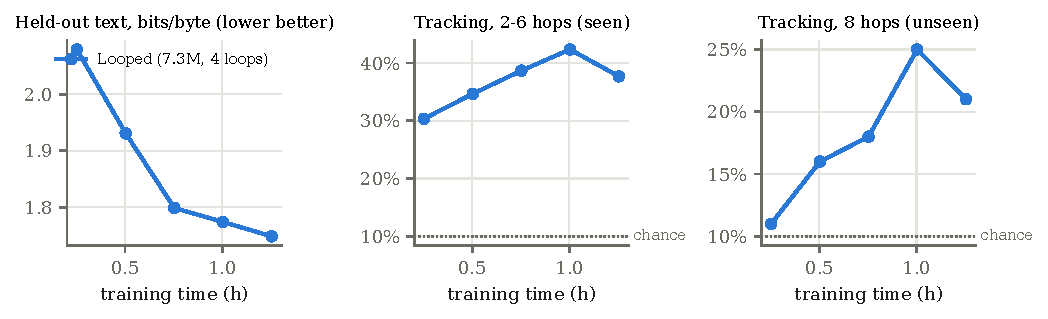
\includegraphics[width=\linewidth]{figures/curves.pdf}}{}
\caption{Training curves (quick evaluation, 100 problems per depth).}
\label{fig:curves}
\end{figure}

\subsection{The agent swarm}\label{sec:swarm}
DRAFT

\section{Discussion and limitations}
DRAFT


\paragraph{Reproducibility.} Code, the agent program, the full experiment ledger, every training curve
and the script that produces every number and figure in this paper are at
\url{https://github.com/jchacker5/inkling-autoresearch}. Numbers in the text are generated from the raw
results by \texttt{paper/make\_figures.py}; none are typed by hand.

\paragraph{Acknowledgements.} Experiments in Section~\ref{sec:swarm} were proposed, implemented and run
by autonomous Claude Code agents following \texttt{program.md}; the harness, the controls and this paper
were built with AI assistance and checked by the author. The research loop follows Karpathy's
autoresearch~\cite{karpathy2026autoresearch}.

\bibliographystyle{plainnat}
\bibliography{refs}

\appendix
\section{Full experiment ledger}
DRAFT

\end{document}
